\documentclass{article}

\pdfminorversion=4

\usepackage{tikz}
\usetikzlibrary{fit,patterns,decorations.pathreplacing}

\usepackage{graphicx}

\def\thindivider{\centerline{\tiny%%
-- --- --- -- ~~~ --- --- --- ~~~ --- -- --- -- ~~~~~~
--- --- --- ~~~  -- --- -- ~~~~~~
--- --- -- ~~~ --- ~~~ -- -- --- -- ~~~ --- --- ---}}

\begin{document}

\title{This PDF is a Git Repository\\Containing its Own \LaTeX\ Source\\and a Copy of Itself}
\author{Evan Sultanik}
\date{April 11, 2017}

\maketitle

Have you ever heard of the \texttt{git bundle} command? I hadn't. It
bundles a set of Git objects---potentially even an entire
repository---into a single file. Git allows you to treat that file as
if it were a standard Git database, so you can do things like clone a
repo directly from it. Its purpose is to easily sneakernet pushes or
even whole repositories across air gaps.

\thindivider

Neighbors, it's possible to create a PDF that is also a Git
repository.

\begin{center}
\begingroup
\setbox9=\hbox{\footnotesize\verb|Receiving objects: 100% (174/174), 103.48 KiB | 0 bytes/s, done.|}
\begin{minipage}{\wd9}
\footnotesize\begin{verbatim}
$ git clone article.pdf foo
Cloning into 'foo'...
Receiving objects: 100% (174/174), 103.48 KiB | 0 bytes/s, done.
Resolving deltas: 100% (100/100), done.
$ cd foo
$ ls
article.pdf article.tex
\end{verbatim}
\end{minipage}
\endgroup
\end{center}

\section{The Git Bundle File Format}
\label{sec:GitBundleFormat}

The file format for Git bundles doesn't appear to be formally
specified anywhere, however, inspecting \texttt{bundle.c} reveals that
it's relatively straightforward:
\def\returnkey{\hspace*{1pt}{\setbox9=\hbox{$\hookleftarrow$}\tikz\node[text width=\wd9,fill=lightgray,rounded corners=1pt] at (0,0){$\hookleftarrow$};}\hspace*{1pt}}
\begin{center}
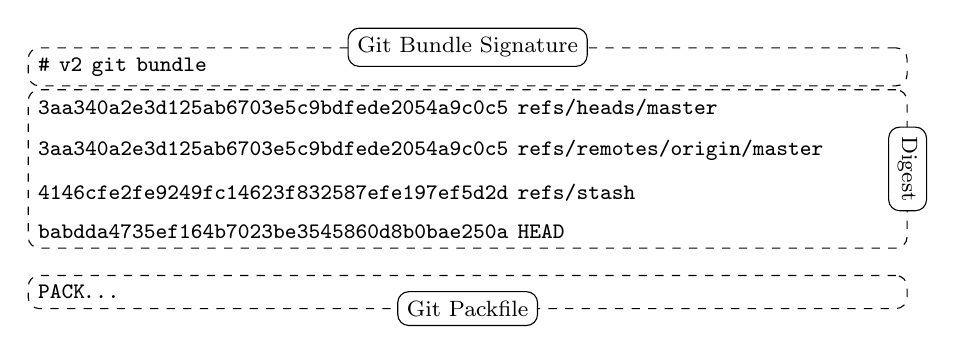
\begin{tikzpicture}
  \node[text width=0.9\hsize] at (0,0) (sig) {\footnotesize\tt\# v2 git bundle{\tiny\returnkey}};
  \node[inner sep=0mm,fit=(sig),draw,rounded corners,dashed,minimum width=0.9\hsize] (sigbox) {};
  \node[draw,rounded corners,fill=white] at (sigbox.north) (siglabel) {\footnotesize Git Bundle Signature};
  \node[text width=0.9\hsize,anchor=north west,yshift=-0.5mm] at (sig.south west) (b1) {\footnotesize\tt 3aa340a2e3d125ab6703e5c9bdfede2054a9c0c5 refs/heads/master{\tiny\returnkey}};
  \node[text width=0.9\hsize,anchor=north west,yshift=-0.5mm] at (b1.south west) (b2) {\footnotesize\tt 3aa340a2e3d125ab6703e5c9bdfede2054a9c0c5 refs/remotes/origin/master{\tiny\returnkey}};
  \node[text width=0.9\hsize,anchor=north west,yshift=-0.5mm] at (b2.south west) (b3) {\footnotesize\tt 4146cfe2fe9249fc14623f832587efe197ef5d2d refs/stash{\tiny\returnkey}};
  \node[text width=0.9\hsize,anchor=north west,yshift=-0.5mm] at (b3.south west) (b4) {\footnotesize\tt babdda4735ef164b7023be3545860d8b0bae250a HEAD{\tiny\returnkey}};
  \node[inner sep=0mm,fit=(b1) (b4),draw,rounded corners,dashed,minimum width=0.9\hsize] (digestbox) {};
  \node[rotate=-90,draw,rounded corners,fill=white] at (digestbox.east) {\footnotesize Digest};
  \node[text width=0.9\hsize,anchor=north west,yshift=-0.5mm] at (b4.south west) (empty) {{\tiny\returnkey}\footnotesize\ };
  \node[text width=0.9\hsize,anchor=north west,yshift=-0.5mm] at (empty.south west) (pack) {{\footnotesize\tt PACK}$\ldots$};
  \node[inner sep=0mm,fit=(pack),draw,rounded corners,dashed,minimum width=0.9\hsize] (packbox) {};
  \node[draw,rounded corners,fill=white] at (pack.south) {\footnotesize Git Packfile};
\end{tikzpicture}
\end{center}
Git has another custom format called a \emph{Packfile} that it uses to
compress the objects in its database, as well as to reduce network
bandwidth when pushing and pulling. The packfile is therefore an
obvious choice for storing objects inside bundles. This of course
raises the question: What is the format for a Git Packfile?

Git does have some internal documentation in
\begin{center}
  \texttt{Documentation/technical/pack-format.txt}
\end{center}
however, it is rather sparse, and does not provide enough detail to
fully parse the format. The documentation also has some
``observations'' that suggest it wasn't even written by the file
format's creator and instead was written by a developer who was later
trying to make sense of the code.

Luckily, Aditya Mukerjee already had to reverse engineer the file
format for his GitGo clean-room implementation of Git, and he wrote an
excellent blog entry about
it\footnote{\texttt{https://codewords.recurse.com/issues/three/unpacking-git-packfiles}}.

\begin{center}
{\small
\def\char#1{\,`\texttt{#1}'\,}
\setbox9=\hbox{\char{K}}
\newdimen\bytewidth\bytewidth=\wd9
\def\byte#1{\hbox to \bytewidth{\hfil\texttt{#1}\hfil}}
\def\desc#1#2{\hbox to #1\bytewidth{\hfil #2\hfil}}
\def\underbrace#1{\draw [
    thick,
    decoration={
        brace,
        mirror,
        raise=2pt
    },
    decorate
] ([xshift=1pt]#1.base west) -- ([xshift=-1pt]#1.base east) 
node (#1label) [pos=0.5,anchor=north,yshift=-2pt]}
\begin{tikzpicture}
\node[inner sep=0pt,minimum width=4\bytewidth] at (0,0) (pack) {\char{P}\char{A}\char{C}\char{K}};
\node[inner sep=0pt,anchor=base west] at (pack.base east) (version) {\byte{00}\byte{00}\byte{00}\byte{02}};
\node[inner sep=0pt,anchor=base west] at (version.base east) (numobj) {\desc{4}{\# objects}};
\underbrace{pack}{\tiny magic};
\underbrace{version}{\tiny version};
\underbrace{numobj}{\tiny big-endian 4 byte int};
\node[inner sep=0pt,anchor=north west] at (packlabel.south -| pack.west) (chunks) {one data chunk for each object};
\node[inner sep=0pt,anchor=north west] at ([yshift=-0.5\baselineskip]chunks.south west) (sha1) {20-byte SHA-1 of all the previous data in the pack};
\end{tikzpicture}}
\end{center}

Although not entirely required to understand the polyglot, I think it
is useful to describe the git packfile format here, since it is not
well documented elsewhere. If that doesn't interest you, it's safe to
skip to the next section.  But if you do proceed, I hope you like
Soviet holes, dear neighbor, because chasing this rabbit might remind
you of \raisebox{-0.5pt}{\includegraphics{kolskaya}}.

\begin{center}
\includegraphics[width=0.33\hsize]{RazvodityeKrolikov_small}
\end{center}

Right, the next step is to figure out the ``chunk'' format.  The chunk
header is variable length, and can be as small as one byte. It encodes
the object's type and its \emph{uncompressed} size. If the object is
a \textit{delta} (\textit{i.e.}, a diff, as opposed to a complete
object), the header is followed by either the SHA-1 hash of the base
object to which the delta should be applied, or a byte reference
within the packfile for the start of the base object. The remainder of
the chunk consists of the object data, zlib-compressed.

This is the format of the variable length chunk header:
\begin{center}
{\newcount\bitnum\bitnum=0
\begin{tikzpicture}
\node[coordinate] at (0,0) (b0) {};
\foreach \i in {1,0,1,1,0,1,0,0,1,1,0,1,0,1,1,0,0,1,0,0,1,0,0,1} {
  {\newcount\prevbit\prevbit=\bitnum
  \global\advance\bitnum by 1
  \node[anchor=west] at (b\the\prevbit.east) (b\the\bitnum) {\i};}
  \draw ([xshift=1pt]b\the\bitnum.south west) -- ([xshift=-1pt]b\the\bitnum.south east);
}
\draw [
    thick,
    decoration={
        brace,
        mirror,
        raise=-2pt
    },
    decorate
] ([xshift=-1pt]b8.north east) -- ([xshift=1pt]b1.north west)
node [pos=0.5,anchor=south,yshift=-2pt] {\footnotesize first byte};
\draw [
    thick,
    decoration={
        brace,
        mirror,
        raise=-2pt
    },
    decorate
] ([xshift=-1pt]b16.north east) -- ([xshift=1pt]b9.north west)
node [pos=0.5,anchor=south,yshift=-2pt] {\footnotesize second byte};
\draw [
    thick,
    decoration={
        brace,
        mirror,
        raise=-2pt
    },
    decorate
] ([xshift=-1pt]b24.north east) -- ([xshift=1pt]b17.north west)
node [pos=0.5,anchor=south,yshift=-2pt] {\footnotesize third byte};

\draw [
    thick,
    decoration={
        brace,
        mirror,
        raise=2pt
    },
    decorate
] ([xshift=1pt]b2.south west) -- ([xshift=-1pt]b4.south east)
node [pos=0.5,yshift=-2pt,anchor=north] (type) {\footnotesize object type};

\draw[<-] ([yshift=-2pt]b1.south) -- (type.south -| b1) node[anchor=north,align=center,font=\footnotesize] {if the MSB is one,\\then this is not\\the last byte};

\draw [
    thick,
    decoration={
        brace,
        mirror,
        raise=2pt
    },
    decorate
] ([xshift=1pt]b5.south west) -- ([xshift=-1pt]b8.south east)
node [pos=0.5,yshift=-2pt,anchor=north,align=center,font=\footnotesize] (length) {first four\\bits of\\the length\\(big-endian)};

\draw[<-] ([yshift=-2pt]b9.south) -- (length.south -| b9) node[anchor=north,align=center,font=\footnotesize] {MSB is one,\\so this is \emph{not} the last byte};

\draw [
    thick,
    decoration={
        brace,
        mirror,
        raise=2pt
    },
    decorate
] ([xshift=1pt]b10.south west) -- ([xshift=-1pt]b16.south east)
node [pos=0.5,yshift=-2pt,anchor=north,align=center,font=\footnotesize] (next) {the next seven\\bits of the length\\(big-endian)};

\draw[<-] ([yshift=-2pt]b17.south) -- (next.south -| b17) node[anchor=north,align=center,font=\footnotesize] {MSB is zero,\\so this \emph{is} the last byte};

\draw [
    thick,
    decoration={
        brace,
        mirror,
        raise=2pt
    },
    decorate
] ([xshift=1pt]b18.south west) -- ([xshift=-1pt]b24.south east)
node [pos=0.5,yshift=-2pt,anchor=north,align=center,font=\footnotesize] {the next seven\\bits of the length\\(big-endian)};

\end{tikzpicture}}
\end{center}
The second through fourth most significant bits of the first byte are
used to store the object type. The remainder of the bytes in the
header are of the same format as bytes two and three in this
example. This example header represents an object of type $11_2$,
which happens to be a git blob, and an \emph{uncompressed} length of
$(100_2\,\verb|<<|\,14) + (1010110_2\,\verb|<<|\,7) + 1001001_2 =
76$,617 bytes.  Since this is not a delta object, it is immediately
followed by the zlib-compressed object data. The header does not
encode the \emph{compressed} size of the object, since the DEFLATE
encoding can determine the end of the object as it is being
decompressed.

At this point, if you found The Life and Opinions of Tristram Shandy
to be boring or frustrating, then it's probably best to skip to the
next section, 'cause it's turtles all the way down.

{\fontfamily{jkpvos}\selectfont\begin{center}
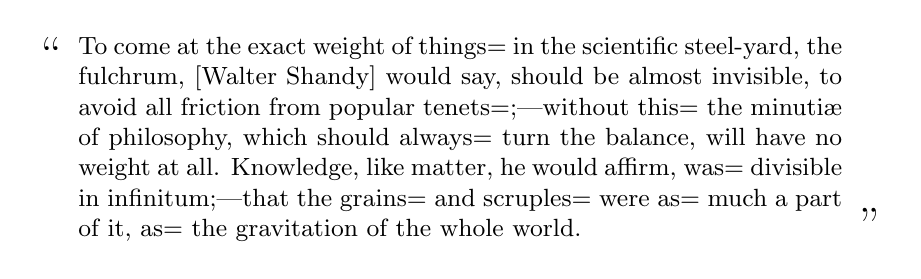
\begin{tikzpicture}
\node at (0,0) (text) {\begin{minipage}{0.8\hsize}\small
To come at the exact weight of things= in the scientific steel-yard, the fulchrum, [Walter Shandy] would say, should be almost invisible, to avoid all friction from popular tenets=;---without this= the minuti\ae\ of philosophy, which should always= turn the balance, will have no weight at all. Knowledge, like matter, he would affirm, was= divisible in infinitum;---that the grains= and scruples= were as= much a part of it, as= the gravitation of the whole world.
\end{minipage}};
\node[anchor=north east] at (text.north west) {\LARGE``};
\node[anchor=south west] at (text.south east) {\LARGE''};
\end{tikzpicture}
\end{center}}

There are two types of delta objects: \emph{references}~(object
type~7) and \emph{offsets}~(object type~6).  Reference delta objects
contain an additional 20~bytes at the end of the header before the
zlib-compressed delta data. These 20~bytes contain the SHA-1 hash of
the base object to which the delta should be applied.  Offset delta
objects are exactly the same, however, instead of referencing the base
object by its SHA-1 hash, it is instead represented by a negative byte
offset to the start of the object within the pack file.  Since a
negative byte offset can typically be encoded in two or three bytes,
it's significantly smaller than a 20-byte SHA-1 hash.  One must
understand how these offset delta objects are encoded if---say, for
some strange, masochistic reason---one wanted to change the order of
objects within a packfile, since doing so would break the negative
offsets. (Foreshadowing!)

One would
\emph{think} that git would use the same multi-byte length encoding that they
used for the uncompressed object length.  But no! This is what we have
to go off of from the git documentation:
\begin{center}
\begingroup
\setbox9=\hbox{\footnotesize\verb|for n >= 2 adding 2^7 + 2^14 + ... + 2^(7*(n-1))|}
\begin{minipage}{\wd9}
\footnotesize\begin{verbatim}
n bytes with MSB set in all but the last one.
The offset is then the number constructed by
concatenating the lower 7 bit of each byte, and
for n >= 2 adding 2^7 + 2^14 + ... + 2^(7*(n-1))
to the result.
\end{verbatim}
\end{minipage}
\endgroup
\end{center}
Right. Some experimenting resulted in the following decoding logic
that appears to work:
\begin{center}
\begingroup
\setbox9=\hbox{\footnotesize\verb|        reference += (1 << (7 * (bytes_read - 1)))|}
\begin{minipage}{\wd9}
\footnotesize
{\color{blue}\verb|def|}\verb| decode_obj_ref|{\color{gray}\verb|(|}\verb|data|{\color{gray}\verb|):|}\\
\verb|    bytes_read = 0|\\
\verb|    reference = 0|\\
\verb|    |{\color{blue}\verb|for|}\verb| c |{\color{blue}\verb|in map|}{\color{gray}\verb|(|}\verb|ord, data|{\color{gray}\verb|):|}\\
\verb|        bytes_read += 1|\\
\verb|        reference <<= 7|\\
\verb|        reference += c & 0b01111111|\\
\verb|        |{\color{blue}\verb|if not|}\verb| |{\color{gray}\verb|(|}\verb|c & 0b10000000|{\color{gray}\verb|):|}\\
{\color{blue}\verb|            break|}\\
{\color{blue}\verb|    if|}\verb| bytes_read >= 2|{\color{gray}\verb|:|}\\
\verb|        reference += |{\color{gray}\verb|(|}\verb|1 << |{\color{gray}\verb|(|}\verb|7 * |{\color{gray}\verb|(|}\verb|bytes_read - 1|{\color{gray}\verb|)))|}\\
{\color{blue}\verb|    return|}\verb| reference, bytes_read|\\
\end{minipage}
\endgroup
\end{center}

The rabbit hole is deeper still; we haven't yet discovered the content
of the compressed delta objects, let alone how they are applied to
base objects.  At this point, we have more than sufficient knowledge
to proceed with the PoC, and my canary died ages ago. Aditya Mukerjee
did a good job of explaining the process of applying deltas in his
blog post, so I will stop here and proceed with the polyglot.

\section{A Minimal Polyglot PoC}

We now know that a git bundle is really just a git packfile with an
additional header, and a git packfile stores individual objects using
zlib, which uses the DEFLATE compression algorithm. DEFLATE supports
zero compression, so if we can store the PDF in a single object (as
opposed to it being split into deltas), then we could theoretically
coerce it to be intact within a valid git bundle.

Forcing the PDF into a single object is easy: We just need to add it
to the repo last, immediately before generating the bundle.

Getting the object to be compressed with zero compression is also
relatively easy.  That's because git was built in almost religious
adherence to The UNIX Philosophy: It is architected with hundreds of
sub commands it calls ``plumbing,'' of which the vast majority you
will likely have never heard. For example, you might be aware
that \texttt{git pull} is equivalent to a \texttt{git fetch} followed
by a \texttt{git merge}. In fact, the \texttt{pull} code actually
spawns a new \texttt{git} child process to execute each of those
subcommands. Likewise, the \texttt{git bundle} command spawns
a \texttt{git pack-objects} child process to generate the packfile
portion of the bundle.  All we need to do is inject
the \texttt{-\relax-compression=0} argument into the list of command line
arguments passed to \texttt{pack-objects}.  This is a one-line
addition to \texttt{bundle.c}:\\ {\footnotesize {\color{gray}
\verb|    argv_array_pushl(&pack_objects.args,|\\
\verb|                     "pack-objects", "--all-progress-implied",|}\\
\verb|                     "--compression=0",|\\
{\color{gray}
\verb|                     "--stdout", "--thin", "--delta-base-offset",|\\
\verb|                     NULL);|
}}

Using our patched version of git, every object stored in the bundle
will be uncompressed!
\begin{center}
\begingroup
\setbox9=\hbox{\footnotesize\verb|$ git bundle create article_bundle.pdf --all|}
\begin{minipage}{\wd9}
\footnotesize\begin{verbatim}
$ export PATH=/path/to/patched/git:$PATH
$ git init
$ git add article.pdf
$ git commit article.pdf -m "added"
$ git bundle create polyglot.pdf --all
\end{verbatim}
\end{minipage}
\endgroup
\end{center}
Any vanilla, un-patched version of git will be able to clone a repo
from the bundle. It will also be a valid PDF, since virtually all
PDF readers ignore garbage bytes before and after the PDF.

\section{Generalizing the PoC}

There are, of course, several limitations to the minimal PoC given in
the previous section:
\begin{enumerate}

\item Adobe, being Adobe, will refuse to open the polyglot unless the PDF is version 1.4 or earlier.  I guess it doesn't like some element of the git bundle signature or digest if it's PDF~1.5. Why? Because Adobe, that's why.

\item Leaving the entire Git bundle uncompressed is wasteful if the repo contains other files; really, we only need the PDF to be uncompressed.

\item If the PDF is larger than 65,535 bytes---the maximum size of an uncompressed DEFLATE block---then git will inject 5-byte deflate block headers inside the PDF, likely corrupting it.

\item Adobe will also refuse to open the polyglot unless the PDF is near the beginning of the packfile\footnote{Requiring the PDF header to start near the beginning of a file is common for many, but not all, PDF viewers.}.

\end{enumerate}

The first limitation is easy to fix by instructing \LaTeX\ to produce
a version 1.4~PDF by adding \texttt{\textbackslash pdfminorversion=4}
to the document.

The second limitation is a simple matter of software engineering,
adding a command line argument to the \texttt{git bundle} command that
accepts the hash of the single file to leave uncompressed, and passing
that hash to \texttt{git pack-objects}. I have created a fork of git
with this feature, available here:
\begin{center}
  \texttt{https://github.com/ESultanik/git/tree/UncompressedPack}
\end{center}

As an aside, while fixing the second limitation I discovered that if a
file has multiple PDFs concatenated after one another
(\textit{i.e.},~a git bundle polyglot with multiple uncompressed PDFs
in the repo), then the behavior is viewer-dependent: Some viewers will
render the first PDF, while others will render the last.  That's a fun
way to generate a PDF that displays completely different content in,
say, macOS~Preview versus Adobe.

The third limitation is very tricky, and ultimately why this polyglot
was not used for the PDF of a digital issue of PoC$\|$GTFO. I've a
solution, but it will not work if the PDF contains any objects
(\textit{e.g.}, images) that are larger than 65,535 bytes. A universal
solution would be to break up the image into smaller ones and tile it
back together, but that is not feasible for a document the size of a
PoC$\|$GTFO issue.

DEFLATE headers for uncompressed blocks are very simple: The first
byte encodes whether the following block is the last in the file, the
next two bytes encode the block length, and the last two bytes are the
ones' complement of the length.  Therefore, to resolve this issue, all
we need to do is move all of the DEFLATE headers that zlib created to
different positions that won't corrupt the PDF, and update their
lengths accordingly.

Where can we put a 5-byte DEFLATE header such that it won't corrupt
the PDF? We could use our standard trick of putting it in a PDF object
stream that we've exploited countless times before to enable
PoC$\|$GTFO polyglots. The trouble with that is: Object streams are
fixed-length, so once the PDF is decompressed (\textit{i.e.},~when a
repo is cloned from the git bundle), then all of the 5-byte DEFLATE
headers will disappear and the object stream lengths would all be
incorrect. Instead, I chose to use PDF comments, which start at any
occurrence of the percent sign character~(\%) outside a string or
stream and continue until the first occurrence of a newline.  All of
the PDF viewers I tested don't seem to care if comments include
non-ASCII characters; they seem to simply scan for a
newline. Therefore, we can inject ``\texttt{\%\textbackslash n}''
between PDF objects and move the DEFLATE headers there. The only
caveat is that the DEFLATE header itself can't contain a newline
byte~(\texttt{0x0A}), otherwise the comment would be ended
prematurely.  We can resolve that, if needed, by adding extra spaces
to the end of the comment, increasing the length of the following
DEFLATE block and thus increasing the length bytes in the DEFLATE
header and avoiding the \texttt{0x0A}. The only concession made with
this approach is that PDF Xref offsets in the deflated version of the
PDF will be off by a multiple of 5, due to the removed DEFLATE
headers. Fortunately, most PDF readers can gracefully handle incorrect
Xref offsets (at the expense of a slower loading time), and this will
only affect the PDF contained in the repository, \emph{not} the PDF
polyglot.

As a final step, we need to update the SHA-1 sum at the end of the
packfile~(\textit{q.v.}~Section~\ref{sec:GitBundleFormat}), since we
moved the locations of the DEFLATE headers, thus affecting the hash.

At this point, we have all the tools necessary to create a generalized
PDF/Git Bundle polyglot for \emph{almost} any PDF and git
repository. The only remaining hurdle is that some viewers require
that the PDF occur as early in the packfile as possible. At first, I
considered applying another patch directly to the git source code to
make the uncompressed object first in the packfile. This approach
proved to be very involved, in part due to git's UNIX design
philosophy and architecture of generic code reuse. We're already
updating the packfile's SHA-1 hash due to changing the DEFLATE
headers, so instead I decided to simply reorder the objects
after-the-fact, subsequent to the DEFLATE header fix but before we
update the hash. The only challenge is that moving objects in the
packfile has the potential to break offset delta objects, since they
refer to their base objects via a byte offset within the packfile.
Moving the PDF to the beginning will break any offset delta objects
that occur after the original position of the PDF that refer to base
objects that occur before the original position of the PDF. I
originally attempted to rewrite the broken offset delta objects, which
is why I had to dive deeper into the rabbit hole of the packfile
format to understand the delta object headers (as you saw at the end
of Section~\ref{sec:GitBundleFormat}, if you were brave enough to
finish it). Rewriting the broken offset delta objects is
the \emph{correct} solution, but, in the end, I discovered a much
simpler way.

\begin{center}
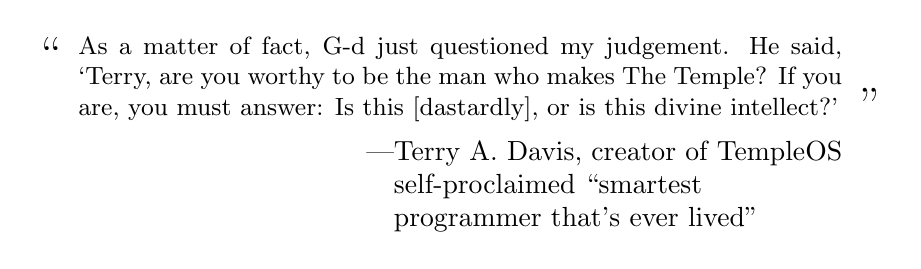
\begin{tikzpicture}
\node at (0,0) (text) {\begin{minipage}{0.8\hsize}\small
As a matter of fact, G-d just questioned my judgement. He said,
`Terry, are you worthy to be the man who makes The Temple? If you are,
you must answer: Is this [dastardly], or is this divine intellect?'
\end{minipage}};
\node[anchor=north east] at (text.north west) {\LARGE``};
\node[anchor=south west] at (text.south east) {\LARGE''};
\node[anchor=north east] at (text.south east) (terry) {\setbox9=\hbox{\llap{---}Terry A.\ Davis, creator of TempleOS}\parbox{\wd9}{\raggedright\box9 self-proclaimed ``smartest programmer that's ever lived''}};
\end{tikzpicture}
\end{center}

Terry's not the only one who's written a compiler!

In the previous section, recall that we created the minimal PoC by
patching the command line arguments to \texttt{pack-objects}.  One of
the command line arguments that is already passed by default
is \texttt{-{}-delta-base-offset}. Running \texttt{git help
pack-objects} reveals the following:
\begin{center}
{\footnotesize\setbox9\hbox{\verb|A packed archive can express the base object of a delta as either a|}
\begin{minipage}{\wd9}
\begin{verbatim}
A packed archive can express the base object of a delta as either a
20-byte object name or as an offset in the stream, but ancient
versions of Git don't understand the latter. By default, git
pack-objects only uses the former format for better compatibility.
This option allows the command to use the latter format for
compactness. Depending on the average delta chain length, this
option typically shrinks the resulting packfile by 3-5 per-cent.
\end{verbatim}
\end{minipage}}
\end{center}
So all we need to do is \emph{remove} the \texttt{-{}-delta-base-offset}
argument and git will not include any offset delta objects in the
pack!

\thindivider

Okay, I have to admit something: There is one more challenge. You see,
the PDF standard~(ISO~32000-1) says
\begin{center}
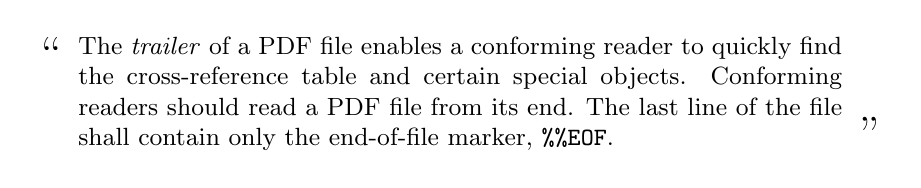
\begin{tikzpicture}
\node at (0,0) (text) {\begin{minipage}{0.8\hsize}\small
The \emph{trailer} of a PDF file enables a conforming reader to
quickly find the cross-reference table and certain special
objects. Conforming readers should read a PDF file from its end. The
last line of the file shall contain only the end-of-file
marker, \texttt{\%\%EOF}.
\end{minipage}};
\node[anchor=north east] at (text.north west) {\LARGE``};
\node[anchor=south west] at (text.south east) {\LARGE''};
\end{tikzpicture}
\end{center}
Granted, we are producing a PDF that conforms to version~1.4 of the
specification, which doesn't appear to have that requirement.
However, at least as early as version 1.3, the specification did have
an implementation note that Acrobat requires the \texttt{\%\%EOF} to
be within the last 1024 bytes of the file.  Either way, that's not
guaranteed to be the case for us, especially since we are moving the
PDF to be at the beginning of the packfile.  There are always going to
be at least 20 trailing bytes after the PDF's \texttt{\%\%EOF} (namely
the packfile's final SHA-1 checksum), and if the git repository is
large, there are likely to be more than 1024 bytes.

Fortunately, most common PDF readers don't seem to care how many
trailing bytes there are, at least when the PDF is version~1.4.
Unfortunately, some readers such as Adobe's try to be ``helpful,''
silently ``fixing'' the problem and offering to save the fixed version
upon exit.  We can at least partially fix the PDF, ensuring that
the \texttt{\%\%EOF} is exactly 20 bytes of the end of the file, by
creating a second uncompressed git object as the very end of the
packfile (right before the final 20~byte SHA-1 checksum).  We could
then move the trailer from the end of the original PDF at the start of
the pack to the new git object at the end of the pack.  Finally, we
could encapsulate the ``middle'' objects of the packfile inside a PDF
stream object, such that they are ignored by the PDF.  The tricky part
is that we would have to know how many bytes will be in that
stream \emph{before} we add the PDF to the git database.  That's
theoretically possible to do \textit{a priori}, but it'd be very labor
intensive to pull off.  Furthermore, using this approach will
completely break the inner PDF that is produced by cloning the
repository, since its trailer will then be in a separate file.
Therefore, I chose to live with Adobe's helpfulness and not pursue
this fix for the PoC.

\thindivider

This PDF is a git bundle containing its \LaTeX\ source, as well as all
of the code necessary to regenerate this polyglot. Clone it to take a
look at the history of this document and its associated code!

{\fontfamily{jkpvos}\selectfont\begin{center}
\begin{minipage}{0.8\hsize}\small
Thus=---thus=, my fellow-neighbours= and associates= in this= great harvest of our learning, now ripening before our eyes=; thus= it is=, by slow steps= of casual increase, that our knowledge physical, metaphysical, physiological, polemical, nautical, mathematical, \ae{}nigmatical, technical, biographical, romantical, chemical, obstetrical, and polyglottical, with fifty other branches= of it, (most of 'em ending as= these do, in ical) have for these four last centuries= and more, gradually been creeping upwards= towards= that Akme of their perfections=, from which, if we may form a conjecture from the advances= of these last \thepage~pages=, we cannot possibly be far off.
\end{minipage}
\end{center}}

\section{License}

Copyright \textcopyright\ 2017 Evan A.~Sultanik

Permission is hereby granted, free of charge, to any person obtaining a copy
of this document and associated source files (the ``Software''), to deal
in the Software without restriction, including without limitation the rights
to use, copy, modify, merge, publish, distribute, sublicense, and/or sell
copies of the Software, and to permit persons to whom the Software is
furnished to do so, subject to the following conditions:

The above copyright notice, this permission notice, and the entire
contents and history of its associated git repository shall be
included in all copies or substantial portions of the Software.

\textsc{The Software is provided ``as is'', without warranty of any kind, express or implied, including but not limited to the warranties of merchantability, fitness for a particular purpose and noninfringement. In no event shall the authors or copyright holders be liable for any claim, damages or liability, whether in an action of contract, tort or otherwise, arising from, out of or in connection with the Software or the use or other dealings in the software.}

\end{document}
